\begin{figure}
  \centering
  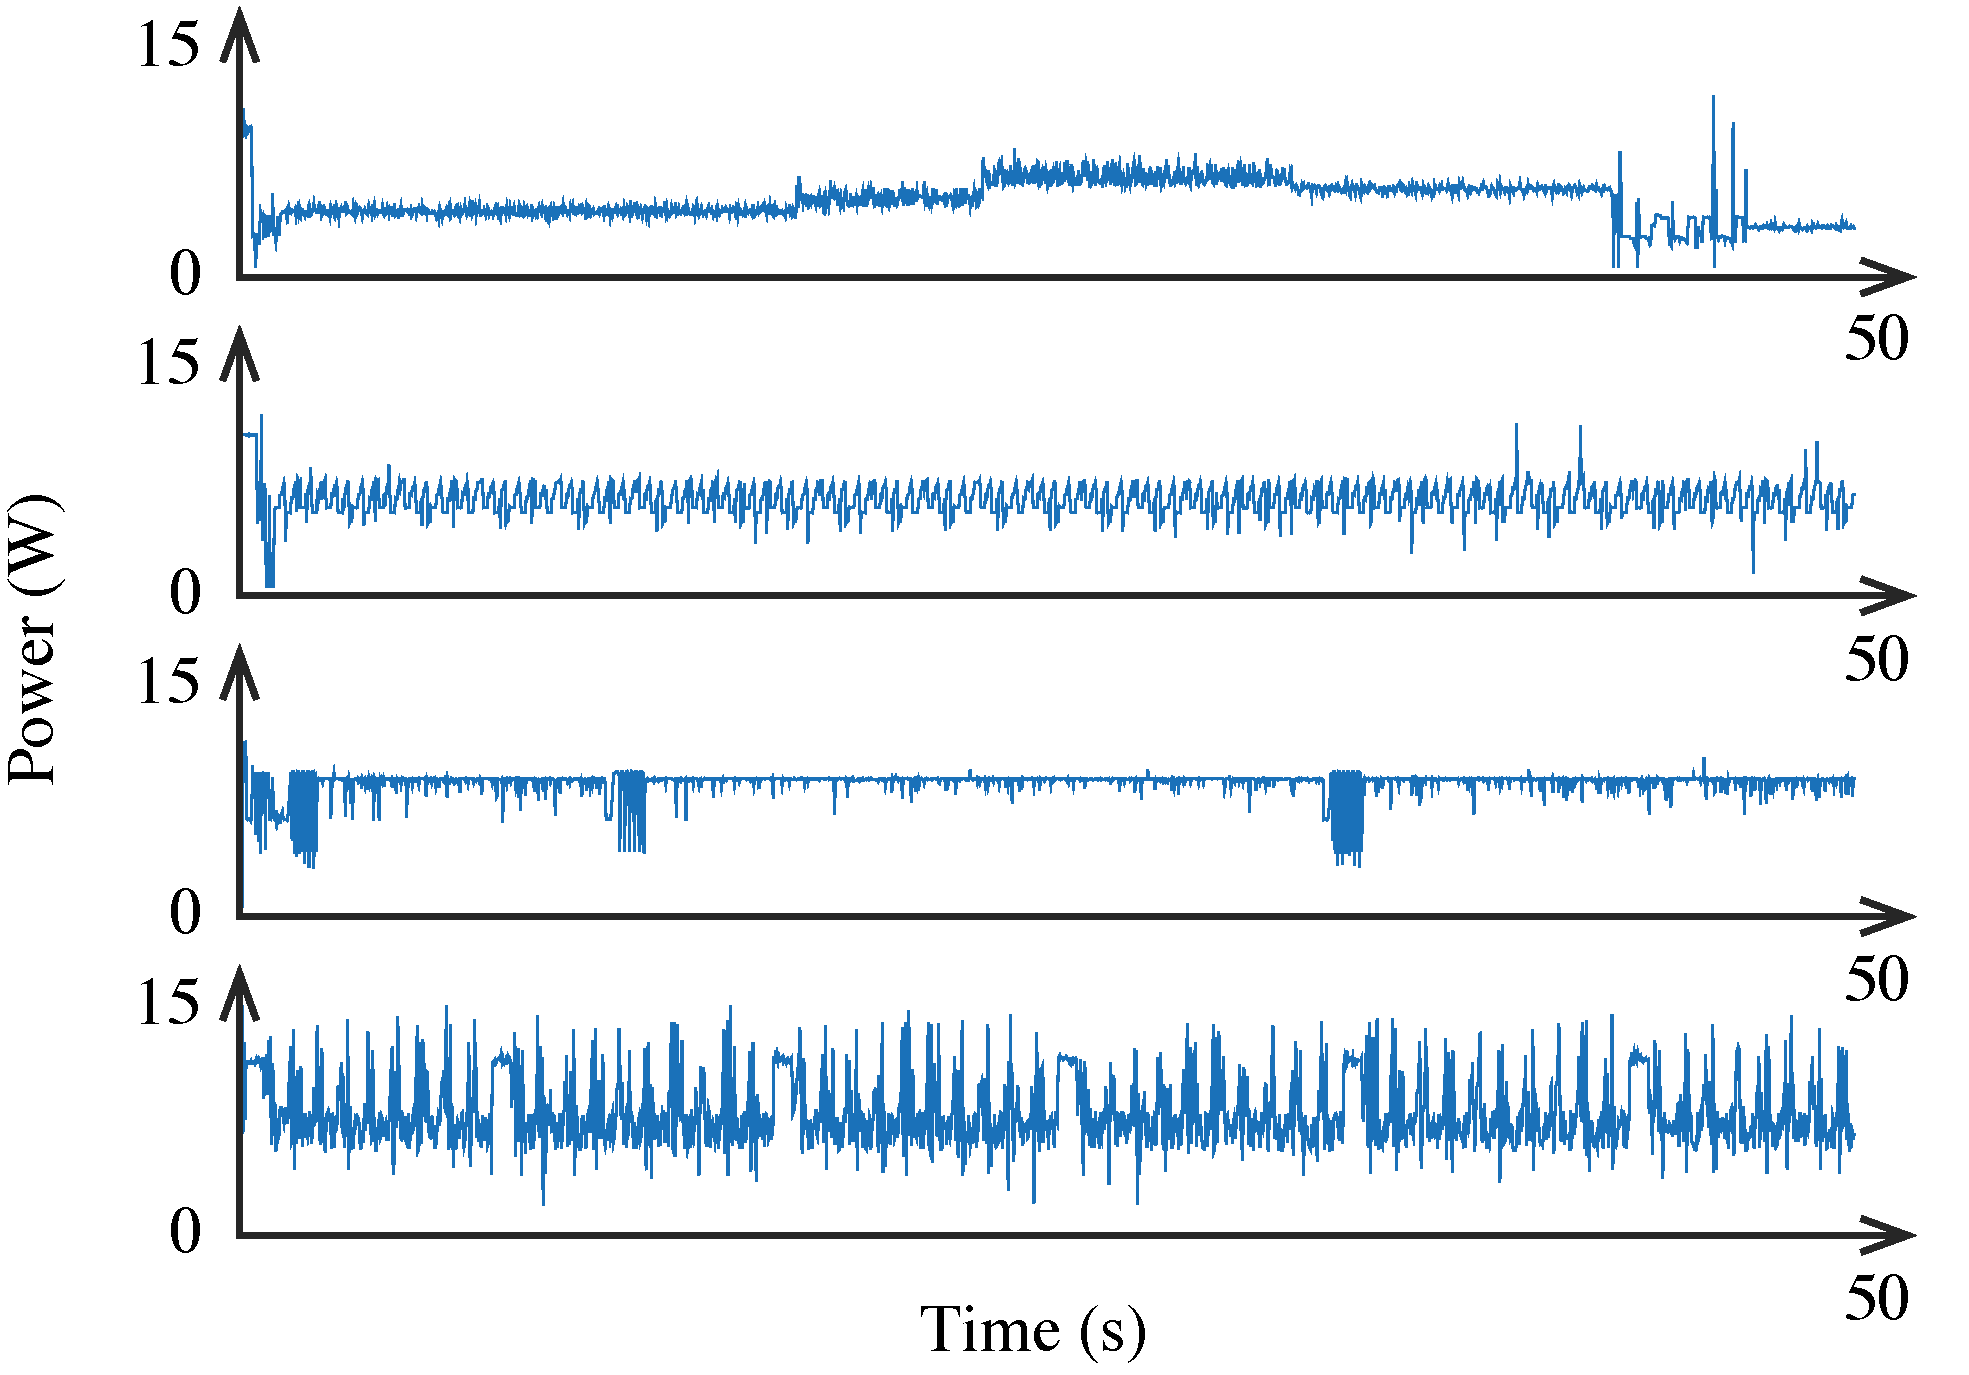
\includegraphics[width=1.0\columnwidth]{include/assets/figures/workload.pdf}
  \caption{
    Power traces of four applications from the \sc{SPEC CPU2006} benchmark
    suite, namely, \tt{astar}, \tt{GemsFDTD}, \tt{bwaves}, and \tt{wrf},
    respectively.
  }
  \flab{workload}
\end{figure}

In the previous subsection, we introduced our approach to generating streams of
arrivals; however, an arrival is only a time stamp without any information about
the actual workload. In this subsection, we describe how workloads needed for
substantiating job arrivals are obtained, which is depicted in the bottom part
of \fref{methodology}. To begin with, workload candidates should conform to a
number of criteria. First, as emphasized throughout the paper, we aim to produce
realistic power and temperature traces, and, therefore, workloads should
represent well the applications or services that the system in question is
supposed to provide to the end user. Second, a workload should be fast to
evaluate, which, in our context, refers to computing the power consumption of
that workload.

The particularities of the power consumption of a computer program are hard to
fabricate. A sequence of random numbers taken out of thin air will not do the
trick as programs have certain algorithmic structures.
Figure~\ref{fig:workload} illustrates the power consumption of four applications
taken from the \sc{SPEC CPU2006} benchmark suite \cite{cpu2006}. A program
might, for instance, traverse a number of phases, and each phase might trigger a
number of distinctive computations, shaping the corresponding power and
temperature profiles. Such features are important to preserve in order to make
the subsequent experimentation with machine-learning techniques and alike
meaningful.

With the above concern in mind, the workload-modeling part of our methodology is
based on full-system simulations of reference programs. However, if we had
incorporated such simulations directly into our workflow, it would have defeated
the purpose of our work since, as motivated in \sref{introduction}, detailed
simulations are too time consuming. Instead, we propose the use of high-level
recordings; see the box labeled ``Recorder'' in \fref{methodology}. To
elaborate, using an adequate simulator capable of modeling the target
architecture, we execute each reference program and record certain information
about this execution.\footnote{Such a technique is similar in spirit to PinPlay
\cite{patil2010}, which is a tool for recording and replaying an execution of a
program on the instruction level.} At a later stage of our pipeline (the box
labeled ``Streamer''), the collected information is utilized in order to flesh
out jobs upon their arrival, and this stage requires no simulation.

From our experience, performance and power simulation is by far the largest
expense on the way to temperature, and, therefore, we propose to record power
directly, eliminating this expense all together. Then the result of the
procedure described above is a repository of power traces corresponding to real
programs, which we refer to as workload patterns (see \fref{methodology}). These
patterns are building blocks: they are used to construct a power profile of the
system under consideration, which we shall further elaborate on in the next
subsection, \sref{performance-model}.

Full-system simulations obviously take time; however, they should be done only
once. Moreover, since researchers tend to test their ideas using similar sets of
benchmark suites and considering similar sets of target architectures, it makes
sense to create a common repository of power patterns that will be populated and
maintained online by the research community. In this case, power patterns will
be at a one-click distance from any single researcher, and no prior simulation
will be needed. The role of such a repository could be similar to the one played
nowadays by the benchmark suites themselves, but it would be on a different
level and for a different purpose.

To recapitulate, we have obtained a set of materials for rendering job arrivals.
These materials, that is, workload patterns, correspond to executions of real
programs and, therefore, possess the particularities found in real life.
